\bluepage{Základní postup kreslení/zobrazovací pipeline}

\begin{frame}
\frametitle{Reprezentace scény}
	\begin{itemize}
		\item{Povrchová reprezentace - vektorová data.}
	\end{itemize}
	\begin{figure}[h]
		\includegraphics[width=10cm,keepaspectratio]{pics/wireframe.jpg}
	\end{figure}
\end{frame}

\begin{frame}
\frametitle{Reprezentace scény}
	\begin{itemize}
		\item{OpenGL pracuje s vrcholy - Vertexy}
		\item{Jeden Vertex může obsahovat několik různých atributů (pozice, barva, čas, hmotnost, texturovací koordináty,...)}
		\item{Několik Vertexů tvoří jedno primitivum - bod, úsečka, trojúhelník,...}
	\end{itemize}
	\begin{figure}[h]
		\includegraphics[width=10cm,keepaspectratio]{pics/primitive.pdf}
	\end{figure}
\end{frame}


\begin{frame}
\frametitle{Zobrazení scény/zobrazovací pipeline}
	\begin{itemize}
		\item Vektorová data se posílají do pipeline a vrací se v podobě rastru
	\end{itemize}
	\begin{picture}(320,250)
		\put(-25,100){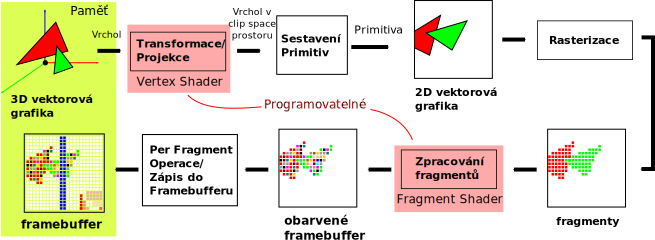
\includegraphics[width=12.5cm,keepaspectratio]{pics/pipeline.pdf}}
	\end{picture}
\end{frame}

\begin{frame}
\frametitle{Programovatelné bloky pipeline}
	\begin{itemize}
		\item V zobrazovací pipeline je několik programovatelných bloků
    \item Vertex Shader blok obsahuje program, který transformuje (přesouvá, promíta vrcholy geometrie)
    \item Vertex Shader často násobí vrcholy maticemi a přesouvá vrcholy mezi několika prostory.
    \item Je pouštěn pro každý vrchol a to paralelně
    \item Fragment Shader blok obsahuje program, který pracuje s fragmenty - vyrasterizovanými úlomky primitiv. Ty často obarvuje.
    \item Fragment Shader je spouštěn alespoň pro každý vyrasterizovaný fragment.
    \item Fragment Shader se také spouští v mnoha instancích, invokacích paralelně.
	\end{itemize}
\end{frame}


\begin{frame}
\frametitle{Matice a prostory}
	\begin{itemize}
		\item Model je namodelovaný v tzn. model space prostoru
    \item Vrcholy modelu se po vynásobení modelovou maticí přesunou do world space prostoru - prostoru scény
    \item Celá scéna se poté transformuje pomocí view matice tak, aby to simulovalo pohled z kamery
    \item Následuje projekce do clip space pomocí projekční matice
    \item Výstup vertex shaderu by měl být v clip space
	\end{itemize}
  \begin{figure}[h]
    \includegraphics[width=10cm,keepaspectratio]{pics/space.pdf}
  \end{figure}
\end{frame}

\begin{frame}
\frametitle{Rasterizace a interpolace}
	\begin{itemize}
		\item Vertexy jsou před rasterizací popsány pomocí n-tice atributů
    \item Rasterizace produkuje fragmenty, pokud jejich střed leží uvnitř primitiva
    \item Po rasterizaci jsou tyto atributy vloženy do fragmetů pomocí interpolace
	\end{itemize}
	\begin{figure}[h]
		\includegraphics[width=10cm,keepaspectratio]{pics/interpolace.pdf}
	\end{figure}
\end{frame}

\begin{frame}
\frametitle{Barycentrické koordináty}
	\begin{figure}[h]
		\includegraphics[width=10cm,keepaspectratio]{pics/barycentrickekoordinaty.pdf}
	\end{figure}
\end{frame}

\begin{frame}
\frametitle{Perspektivní zkreslení}
	\begin{itemize}
		\item Vertex atributy se mohou interpolovat v rovině průmětny nebo v prostoru scény
    \item Aby se mohlo interpolovat v prostoru scény, musí se provést perspektivní korekce
      (v OpenGL automaticky/lze vypnout)
	\end{itemize}
	\begin{figure}[h]
		\includegraphics[width=10cm,keepaspectratio]{pics/prespektivni_korekce.pdf}
	\end{figure}
\end{frame}


